\documentclass[12pt]{article}
\usepackage[left=2cm, top=2cm, right=2cm, bottom=2cm]{geometry}
\usepackage[utf8]{inputenc}
\usepackage[T1]{fontenc}
\usepackage[french]{babel}
\usepackage{graphicx}
\usepackage{graphics}
\usepackage{amsmath}
\usepackage{tikz}
\usepackage{graphicx}
\usepackage{xcolor}
\usepackage{parskip}
\usepackage{physics}
\usepackage{gensymb}

\title{\textbf{Instrumentation} \\ TP 2: Caractérisation d'un capteur de température}
\author{MENARD Alexandre \\ VIEILLEDENT Florent \\ RANCHY Nilo}

\setlength{\parindent}{1cm}

\begin{document}
\maketitle

\section*{Introduction}
Dans ce travail pratique, on étudie les caractéristiques d'un capteur de température PT100. Le capteur est composé notamment d'une couche de platine dont la résistance varie en fonction de la température. Le capteur que nous utilisons est de classe B et de type PTFF.100 fait référence à la résistance $R_0$ du capteur à $0\degree C$. On commence par un circuit d'un pont diviseur de tension. On cherche alors à déterminer la température de la pièce en mesurant la résistance du capteur. On cherche aussi à déterminer le temps de réponse du capteur et on étudie l'influence du courant sur les mesures. On change ensuite le circuit de conditionnement en utilisant un Pont de Wheatstone, pour comparer la sensibilité des deux circuits.

\section{Premier circuit de conditionnement : Pont diviseur de tension}
\subsection{Montage expérimental}
La fiche technique du capteur nous indique un courant recommandé pour nos mesure de $I_{mes}=1.4\, mA$, nous allons donc utiliser un pont diviseur de tension pour avoir le courant voulu dans notre capteur. Notre montage est composé d'un générateur de tension $E=5.0136\, V$ (mesuré avec un voltmètre), d'une résistance $R=5.085 \, k\Omega$(mesuré avec un ohmmètre), d'un voltmètre et du capteur de température. On note respectivement $R_{PT}$ et $U_{PT}$ la résistance du capteur et la tension à ses bornes. 

Pour calculer la température de la pièce, on commence par calculer $R_{PT}$ avec un ohmmètre. Puis on calcule $U_{PT}$ avec le circuit 1 de la figure (\ref{Schéma_exp1}).

Pour mesurer le temps de réponse du capteur, on réutilise le même circuit. On commence par chauffer le capteur en le tenant dans nos doigts. Puis on filme le voltmètre avec un chronomètre à côté et on laisse refroidir le capteur. On note tout les secondes la tension aux bornes du capteur.  

\newpage
\begin{figure}[h!]
	\begin{center}
		\includegraphics[scale=0.1]{Schéma_exp1.png}
		\label{Schéma_exp1}
		\caption{Gauche : Circuit 1 pour mesurer la température de la pièce et calculer le temps de réponse. Droite : Circuit 2 pour déterminer la relation entre l'intensité et la température}
	\end{center}
\end{figure}

On utilise ensuite le circuit 2. On mesure $U_{PT}$ en faisant varier la résistance du potentiomètre $R_{PT}$ de 3500 à 250 $\Omega$.

\subsection{Modèle}
D'après la fiche technique du capteur, on a la relation suivant pour $T\geq 0\degree C$:
\begin{equation}
R_{PT}=R_0(1+a*T+b*T^2)
\end{equation}
avec $a=3.9083*10^{-3}$ et $b=-5.775*10^{-7}$. Dans notre cas, on utilise une approximation linéaire de cette formule:
\begin{equation}
R_{PT}=R_0(1+a*T)
\label{Modèle_linéaire}
\end{equation}

On calcule la différence entre ces deux modèles. On remarque que pour des températures ambiantes (entre $0$ et $40\degree C$), la différence de température entre les deux modèles est inférieur à $0.25\degree C$. On accepte cet écart pour cette première expérience mais il faut le prendre en compte dans nos conclusions. 
\begin{figure}[h!]
	\begin{center}
		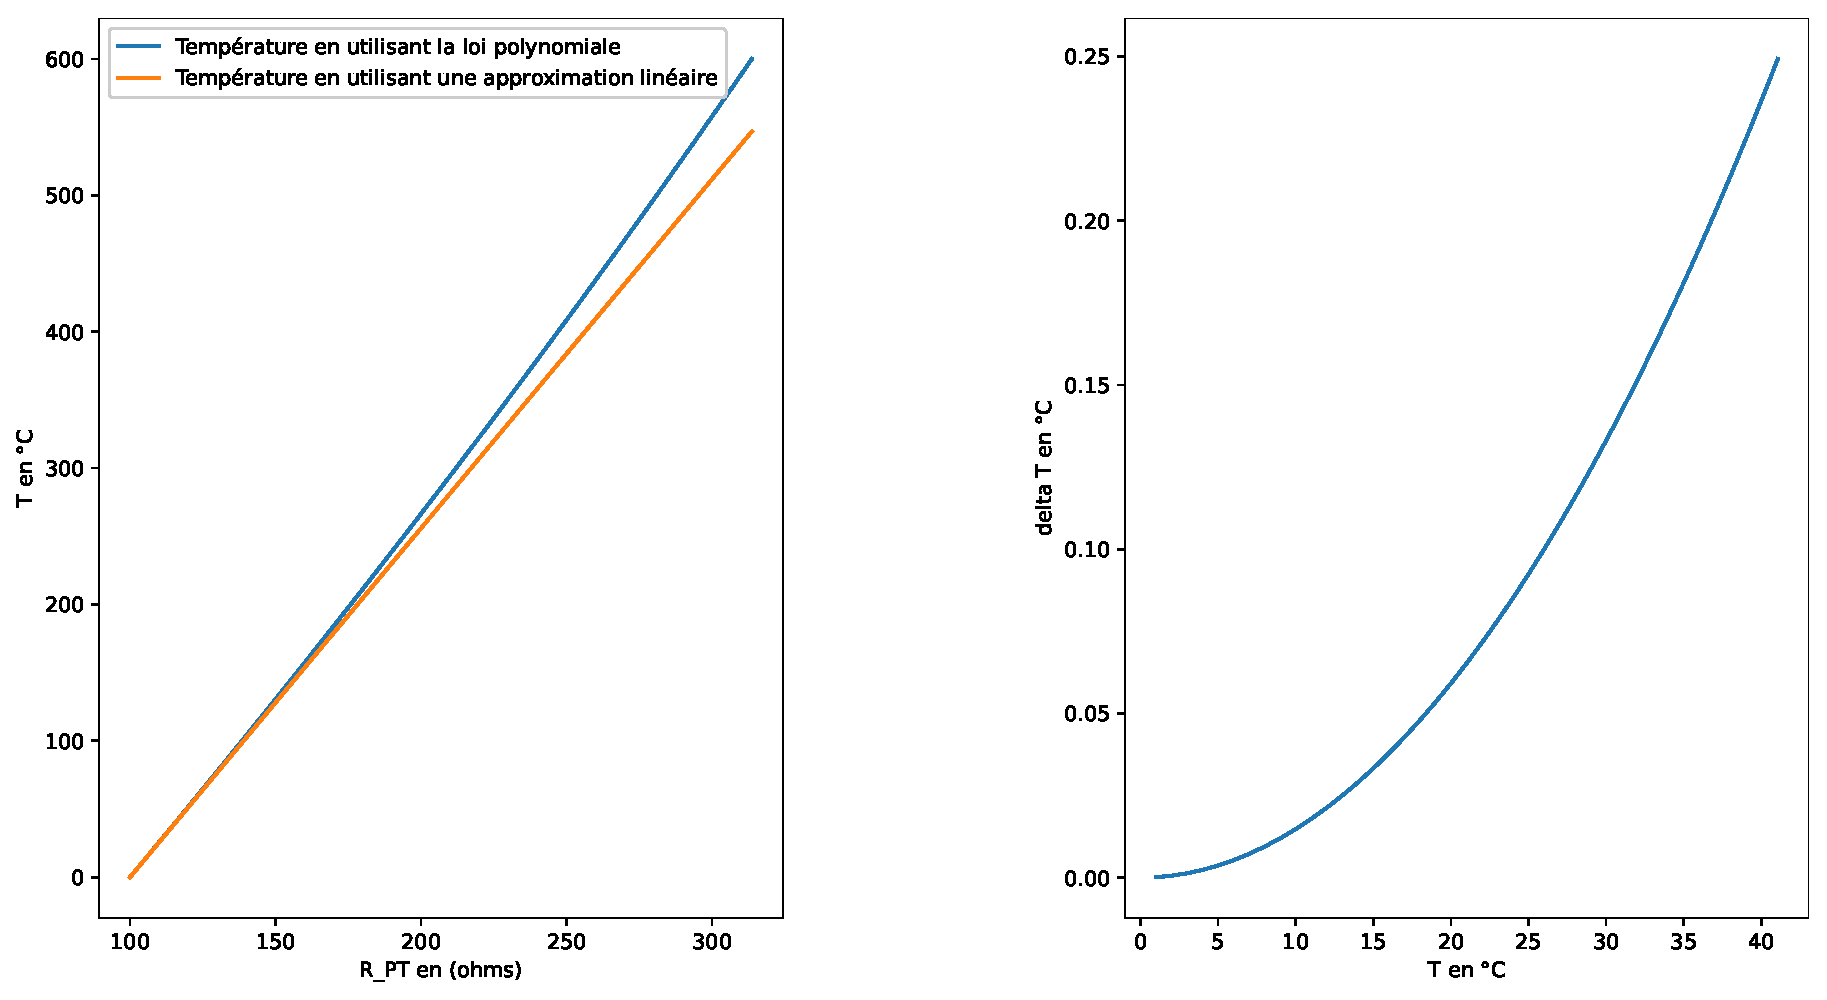
\includegraphics[scale=0.3]{Comparaison.eps}
		\label{Comparaison}
		\caption{Gauche: Comparaison des températures calculées avec les deux modèles. Droite: Différence entre les modèles pour des température ambiantes}
	\end{center}
\end{figure}

D'après l'équation (\ref{Modèle_linéaire}), on a donc la relation suivante:
\begin{equation}
T=\frac{R_{PT}-R_0}{a*R_0}
\label{Equation_température}
\end{equation}

En utilisant la formule du pont diviseur de tension, on trouve la relation entre $R_{PT}$ et $U_{PT}$:
\begin{align}
U_{PT}=\frac{R_{PT}}{R+R_{PT}}E \Rightarrow R_{PT}=\frac{R*U_{PT}}{E-U_{PT}}
\label{Equa_resistance}
\end{align}

Pour calculer l'intensité $i$ qui traverse la capteur : 
\begin{equation}
i=\frac{E}{R+R_{PT}}
\label{Equa_intensité}
\end{equation}

On s'attend à ce que la température suive une loi exponentielle au fil du temps. Si on note $T_A$ la température de la pièce, $T_0$ la température à laquelle on chauffe le capteur et $\tau$ le temps caractéristique du capteur, on a :
\begin{align}
T(t)&=T_A+(T_0-T_A)*e^{-\frac{t}{\tau}}\Rightarrow
(T(t)-T_A)=(T_0-T_A)*e^{-\frac{t}{\tau}}
\label{exponentielle}
\end{align}   

La fiche technique nous donne un $\tau_{0.9}=10\, s$, ce qui correspond à 
\begin{equation}
1-e^{\frac{\tau_{0.9}}{\tau}}=0.9 \Rightarrow \tau_{0.9}=ln(\frac{1}{0.1})*\tau
\label{Equa_tempsréponse}
\end{equation}

Lorsqu'on diminue beaucoup la résistance du potentiomètre, on augmente l'intensité du courant. L'effet Joule va donc augmenter. On rappelle l'expression de l'effet Joule :$P=RI^2$. La fiche technique nous donne un coefficient d'auto-chauffage en $\degree C/mW$, qu'on note $a$. Par analyse dimensionnelle, on a la relation suivante :
\begin{equation}
\delta T=a*10^{3}*P=a*10^{3}*i^2*R_{PT}
\label{Equation_puissance}
\end{equation}



\subsection{Mesures et expérimentation}

On commence par mesurer la température de la pièce. On mesure $U_{PT}=105.97\pm 0.02\, mV$. On fait l'application numérique en utilisant l'équation (\ref{Equa_resistance}) et on trouve $R_{PT}=109.80\, \Omega$. On utilise la méthode de la dérivée pour trouver l'incertitude :
\begin{align*}
\delta R_{PT}&=\frac{dR_{PT}}{dU_{PT}}*\delta U_{PT} \\
\delta R_{PT}&=\frac{R*E}{(E-U_{PT})^2}*\delta U_{PT} \\
\delta R_{PT}&=\frac{5.085.10^{3}*5.0136}{(5.0136-105.97*10^{-3})}*(0.02*10^{-3})\\
\delta R_{PT}&=0.02\, \Omega
\end{align*}

On utilise ensuite l'équation (\ref{Equation_température}) et on obtient $T=25.07 \degree C$. On calcule aussi l'incertitude : $\delta T = \frac{\delta R_{PT}}{a*R_0}=0.05 \degree C$. On a donc $T=25.07\pm 0.05 \degree C$. On a aussi mesuré le température avec un thermocouple et on obtient $T_{thermocouple}=25.0\pm 0.5 \degree C$. Les valeurs sont cohérentes. 
[COMPARAISON OHMMÈTRE]

\newpage
On cherche maintenant à déterminer le temps de réponse. On regroupe les données de tension en fonction du temps dans un tableau:
\begin{table}[!h]
	\begin{center}
		\begin{tabular}{|c|c|}
\hline
 t $\pm 0.1$ (en s) &  $U_{PT}\pm 0.05$ (en mV) \\
\hline
        0 &        110.58 \\
        1 &        110.41 \\
        2 &        109.99 \\
        3 &        109.66 \\
        4 &        109.32 \\
        5 &        109.17 \\
        6 &        109.00 \\
        7 &        108.81 \\
        8 &        108.65 \\
        9 &        108.52 \\
       10 &        108.42 \\
       11 &        108.35 \\
       12 &        108.29 \\
       13 &        108.24 \\
       14 &        108.21 \\
       15 &        108.20 \\
       16 &        108.17 \\
       17 &        108.13 \\
       18 &        108.10 \\
       19 &        108.09 \\
       20 &        108.07 \\
       21 &        108.07 \\
       22 &        108.06 \\
       23 &        108.06 \\
       24 &        108.05 \\
       25 &        108.04 \\
       26 &        108.04 \\
\hline
\end{tabular}
	\end{center}
	\label{Tableau_Data}
	\caption{Données pour calculer le temps de réponse}
\end{table}

\newpage
Grâce aux équations(\ref{Equa_resistance}) et (\ref{Equation_température}), on calcule la température associée à chaque tension. On trace $\Delta T=T-T_A$ en fonction du temps, avec $T_A$ la dernière température mesurée.

\begin{figure}[h!]
	\begin{center}
		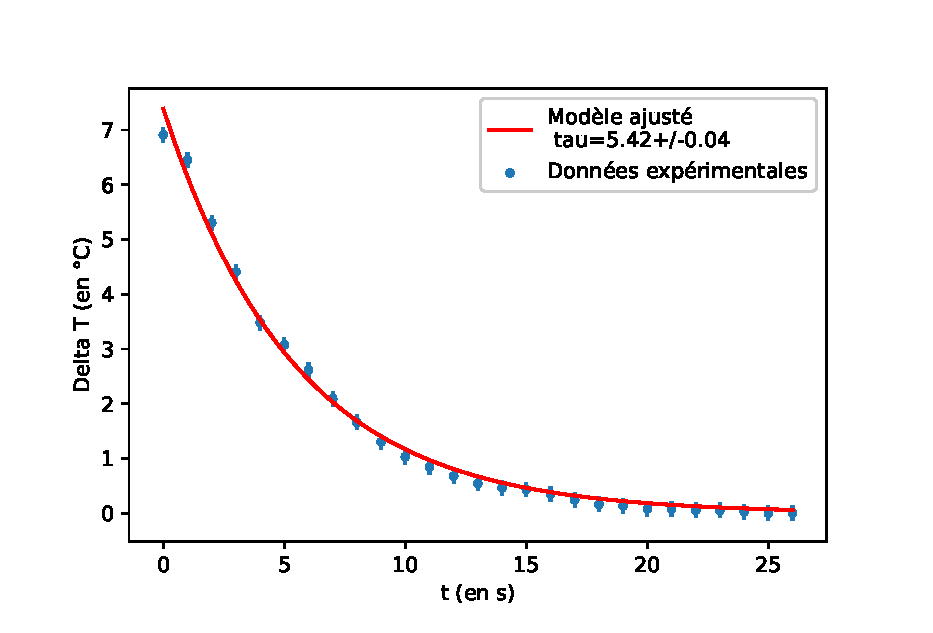
\includegraphics[scale=0.7]{Tempscara.eps}
		\label{Temps_caractéristique}
		\caption{$\Delta T$ en fonction du temps et courbe ajustée}
	\end{center}
\end{figure}

On trouve bien une courbe exponentielle, il y a donc un accord qualitative avec l'équation (\ref{exponentielle}). On ajuste une courbe avec Python et on trouve un $\tau = 5.42\pm 0.04\,s$. Grâce à l'équation (\ref{Equa_tempsréponse}), on calcule notre temps de réponse expérimentale $\tau_{0.9}=12.48\pm 0.09\,s$. [COMPARAISON THEORIQUE AIR FLOW JOUER DE LA FLUTE].



\end{document}
